\textbf{\underline{OZ 6 - Magnetische inductie en de wet van Faraday - Oefening 4:}}
\vspace{0.5cm}
    Bepaal de emf geïnduceerd in een vierkante lus waarbij de lus in rust blijft en een stroom in de rechte draad gegeven is door $I(t) = 15.0\sin(2500t)$ A met $t$ de tijd in seconden. De afstand $a$ is $12.0$ cm, en $b$ is $15.0$ cm.

    \begin{center}
        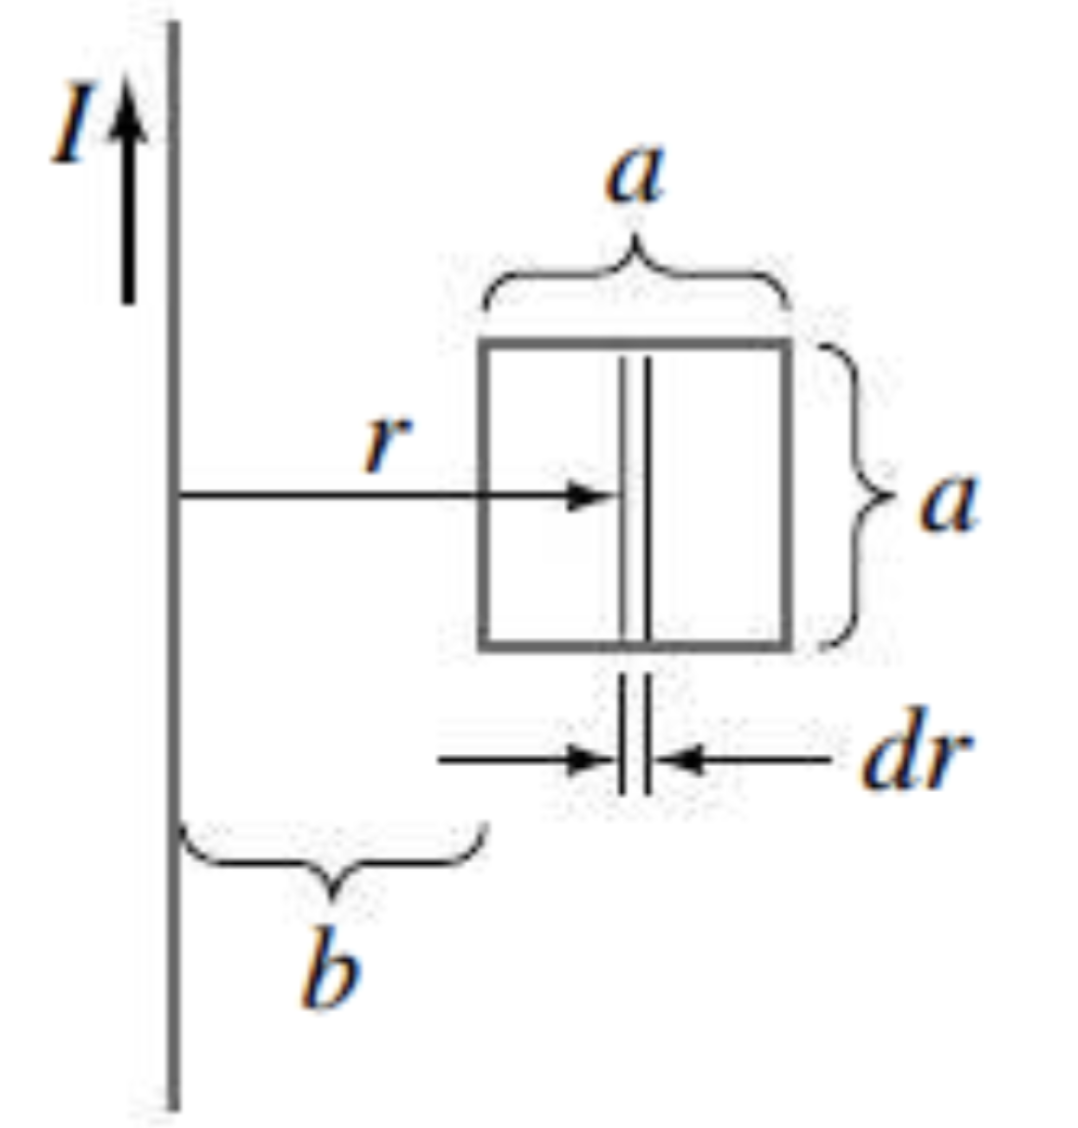
\includegraphics[scale = 0.18]{oz06/resources/Oz6Oef4.png}
    \end{center}

    \begin{description}[labelwidth=1.5cm, leftmargin=!]
        \item[Geg. :]
        \item[Gevr. :] 
        \item[Opl. :]
    \end{description}


\vspace{1cm}